% Figure 2: Migration DAG for §6.
% Nodes: configurations C1-C7. Edges: PQ-ward migrations.
% Edge styles encode blocker class (a/b/c/d) per §6.
% PQ-ready endpoints (C6, C7) are highlighted.
\begin{figure}[t]
  \centering
  \resizebox{\columnwidth}{!}{%
  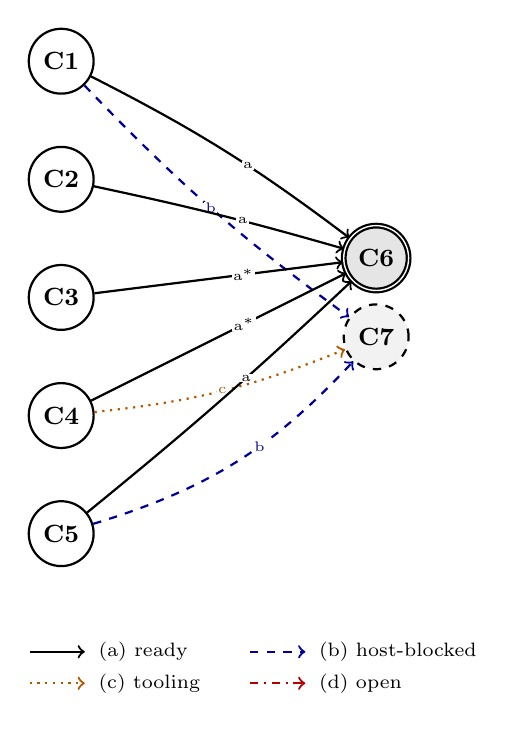
\begin{tikzpicture}[
      cfg/.style={
        circle, draw, thick, minimum size=7mm,
        font=\small\bfseries, fill=white
      },
      pqready/.style={
        cfg, fill=gray!20, double, double distance=0.5pt
      },
      blocked/.style={
        cfg, dashed, fill=gray!10
      },
      ea/.style={->, thick, black},                    % class (a) — solid
      eb/.style={->, thick, dashed, blue!60!black},    % class (b) — host blocked
      ec/.style={->, thick, dotted, orange!70!black},  % class (c) — tooling
      ed/.style={->, thick, dashdotted, red!70!black}, % class (d) — open
      lblstyle/.style={font=\tiny, fill=white, inner sep=0.5pt},
      legend/.style={font=\scriptsize}
    ]
    % Starting configs on the left, PQ-ready destinations on the right.
    \node[cfg]      (C1) at (0,  3.0) {C1};
    \node[cfg]      (C2) at (0,  1.5) {C2};
    \node[cfg]      (C3) at (0,  0.0) {C3};
    \node[cfg]      (C4) at (0, -1.5) {C4};
    \node[cfg]      (C5) at (0, -3.0) {C5};

    \node[pqready]  (C6) at (4.0,  0.5) {C6};
    \node[blocked]  (C7) at (4.0, -0.5) {C7};

    % Migration edges (from §6 prose).
    \draw[ea] (C1) to[bend left=5]   node[lblstyle, pos=0.6] {a}        (C6);
    \draw[eb] (C1) to[bend right=5]  node[lblstyle, pos=0.5] {b}        (C7);
    \draw[ea] (C2) to[bend left=2]   node[lblstyle, pos=0.6] {a}        (C6);
    \draw[ea] (C3) to                node[lblstyle, pos=0.6] {a$^\ast$} (C6);
    \draw[ea] (C4) to                node[lblstyle, pos=0.6] {a$^\ast$} (C6);
    \draw[ec] (C4) to[bend right=8]  node[lblstyle, pos=0.5] {c}        (C7);
    \draw[ea] (C5) to[bend right=2]  node[lblstyle, pos=0.6] {a}        (C6);
    \draw[eb] (C5) to[bend right=15] node[lblstyle, pos=0.6] {b}        (C7);

    % Legend below the diagram.
    \begin{scope}[shift={(2.0, -4.5)}]
      \draw[ea] (-2.4, 0.0) -- (-1.7, 0.0);
        \node[legend, anchor=west] at (-1.65, 0.0) {(a) ready};
      \draw[eb] ( 0.4, 0.0) -- ( 1.1, 0.0);
        \node[legend, anchor=west] at ( 1.15, 0.0) {(b) host-blocked};
      \draw[ec] (-2.4,-0.4) -- (-1.7,-0.4);
        \node[legend, anchor=west] at (-1.65,-0.4) {(c) tooling};
      \draw[ed] ( 0.4,-0.4) -- ( 1.1,-0.4);
        \node[legend, anchor=west] at ( 1.15,-0.4) {(d) open};
    \end{scope}
  \end{tikzpicture}}%
  \caption{Migration paths from each starting configuration toward a
    post-quantum-ready endpoint. C6 (STARK over Goldilocks on a
    FRI-aware anchor) is the deployable PQ-ready destination; C7
    (Stellar + Plonky3 + FRI, dashed) is host-function-blocked. Edge
    styles denote the §6 blocker class. $^\ast$ = the migration is
    technically Class~(a) but loses application-relevant semantics
    (verifier-as-rollup for C3, protocol-level recursion for C4).
    Lattice paths are Class~(d) from every starting configuration
    and are not drawn as individual edges.}
  \label{fig:migration}
\end{figure}
